
% Use only LaTeX2e, calling the article.cls class and 12-point type.
\documentclass[11pt]{article}

\usepackage[english]{babel}

%%ys: allow pdf version 1.6 to avoid the warning message
\pdfoptionpdfminorversion 6

% Users of the {thebibliography} environment or BibTeX should use the
% scicite.sty package, downloadable from *Science* at
% www.sciencemag.org/about/authors/prep/TeX_help/ .
% This package should properly format in-text
% reference calls and reference-list numbers.

\usepackage{scicite}

% Use times if you have the font installed; otherwise, comment out the
% following line.

%\usepackage{times}
%%ys: better looking ttfamily
\renewcommand{\rmdefault}{ptm}

% The preamble here sets up a lot of new/revised commands and
% environments.  It's annoying, but please do *not* try to strip these
% out into a separate .sty file (which could lead to the loss of some
% information when we convert the file to other formats).  Instead, keep
% them in the preamble of your main LaTeX source file.

%% ys: packages not included in original template .tex
\usepackage{graphicx}
\usepackage{caption}
\captionsetup{%
  margin=0.25in,
  font=small,
  labelsep=quad,
  labelfont=bf,
  figurewithin=section,
  tablewithin=section}
\usepackage[usenames,dvipsnames]{color}
%% "colorlinks" disables border
\usepackage[colorlinks,linkcolor=Blue]{hyperref}


% The following parameters seem to provide a reasonable page setup.

\topmargin 0.0cm
\oddsidemargin 0.2cm
\textwidth 16cm
\textheight 21.5cm
\footskip 1.0cm


%The next command sets up an environment for the abstract to your paper.

\newenvironment{sciabstract}{%
\begin{quote} \bf}
{\end{quote}}


% If your reference list includes text notes as well as references,
% include the following line; otherwise, comment it out.

\renewcommand\refname{References and Notes}


\newcounter{lastnote}
\newenvironment{scilastnote}{%
\setcounter{lastnote}{\value{enumiv}}%
\addtocounter{lastnote}{+1}%
\begin{list}%
{\arabic{lastnote}.}
{\setlength{\leftmargin}{.22in}}
{\setlength{\labelsep}{.5em}}}
{\end{list}}


% Include your paper's title here

\title{Latent structure in random sequences drives neural learning toward a rational bias}




\author
{Yanlong Sun$^{1\dagger}$, Randall C. O'Reilly$^{2}$, Rajan Bhattacharyya$^3$,\\
Jack W. Smith$^4$, Xun Liu$^5$, Hongbin Wang$^{6\dagger}$\\
\\
\normalsize{$^{1,4,6}$ Texas A\&M University Health Science Center}\\
\normalsize{$^{2}$ Department of Psychology and Neuroscience, University of Colorado Boulder} \\
\normalsize{$^{3}$ Center for Neural and Emergent Systems, HRL Laboratories, LLC} \\
\normalsize{$^{5}$ Institute of Psychology, Chinese Academy of Sciences} \\
\\
\normalsize{$^\dagger$To whom correspondence should be addressed}\\
\normalsize{E-mail:  ysun@tamhsc.edu, hwang@tamhsc.edu}
}

% Include the date command, but leave its argument blank.

\date{}



%%%%%%%%%%%%%%%%% END OF PREAMBLE %%%%%%%%%%%%%%%%



\begin{document}

% Double-space the manuscript.
%\baselineskip24pt
%%ys: 1.5-space the manuscript.
\baselineskip18pt

% Make the title.

\maketitle



% Place your abstract within the special {sciabstract} environment.

\begin{sciabstract}
People generally fail to produce random sequences by overusing alternating patterns and avoiding repeating ones --- the {\em gambler's fallacy} bias.
We offer a novel account for the neural basis of this bias, based on a biologically-motivated neural model that learns from errors in predicting what will happen next.  When applied to random sequences over time, the model naturally develops a representation that is biased toward alternation, because of its sensitivity to some surprisingly rich statistical structure that emerges in these random sequences.
Furthermore, the model directly produces the best-fitting bias parameter for an existing Bayesian model, by which we obtain an accurate fit to the human data in random sequence production.  These results show that our seemingly irrational, biased view of randomness can be understood instead as the perfectly reasonable response of an effective learning mechanism to subtle statistical structure embedded in random sequences.
\end{sciabstract}

There is a surprising amount of systematic structure lurking within random sequences.
For example, in the classic case of flipping a fair coin, where the probability of each outcome (Heads or Tails) is exactly $0.5$ on every single trial, one would naturally assume that there is no possibility for some kind of interesting structure to emerge, given such a simple and extreme, desolate form of randomness.
And yet, if one records the average amount of time it takes for a repetition (\texttt{HH} or \texttt{TT}) to first occur in a sequence (the \emph{waiting time} statistic), it is significantly longer ($6$ tosses) than for an alternation (\texttt{HT} or \texttt{TH}, $4$ tosses).
This is despite the fact that, on average, repetitions and alternations are equally probable --- as one would expect, occurring once in every $4$ tosses (the \emph{mean time} statistic).
For both of these facts to be true, it must be that repetitions are more bunched together over time --- they come in bursts, with greater spacing between, compared to alternations.
Intuitively, this difference comes from the fact that repetitions can build upon each other (e.g., \texttt{HHH} contains $2$ repetitions of \texttt{HH}), whereas alternations cannot.
Another source of insight comes from the transition graph (\textbf{Figure~1A}), which reveals a structural asymmetry in the process of fair coin flipping:
the number of transitions it takes to leave then revisit a repetition state is longer than that for an alternation state.
%(This is in fact the definitions of waiting time: the waiting has to \emph{start from scratch}.)
As a consequence, with $p_A$ denoting the \emph{probability of alternation} between any two consecutive trials,
repetitions will have longer waiting times than alternations as long as $p_A > 1/3$, in spite of the same mean time at $p_A = 1/2$ (\textbf{Figure~1B}).


\begin{figure}[h!t]
  \centering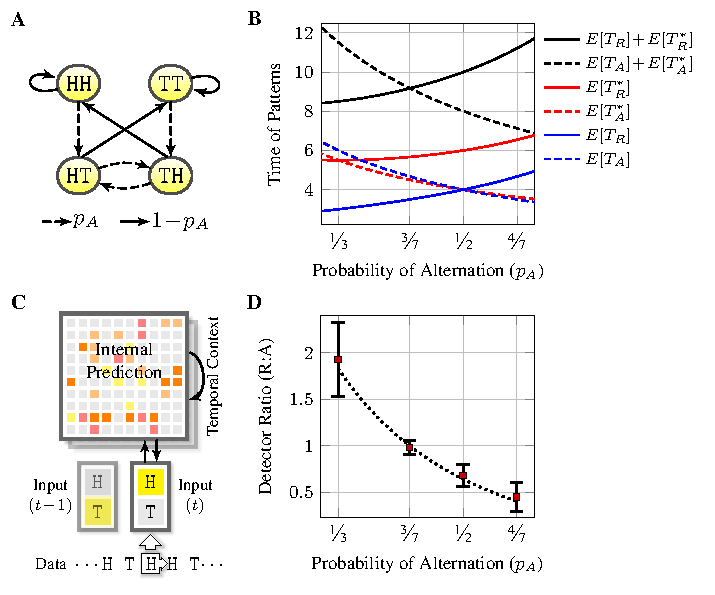
\includegraphics[scale=1]{RND-Figs/Fig1}
  \caption{\textbf{A}. Transitions between patterns of length $2$ described by the probability of alternation between consecutive trials ($p_A$).
  At $p_A\!=\!1/2$, the process has the same chance to enter or leave either a repetition (\texttt{HH} or \texttt{TT}) or an alternation (\texttt{HT} or \texttt{TH}) state.
  However, it takes a minimum of $3$ transitions for the process to leave then revisit a repetition state (e.g., \texttt{HH} $\rightarrow$ \texttt{HT} $\rightarrow$ \texttt{TH} $\rightarrow$ \texttt{HH}), but only $2$ for an alternation state (e.g., \texttt{HT} $\rightarrow$ \texttt{TH} $\rightarrow$ \texttt{HT}).
  \textbf{B}. Equilibriums by $p_A$ values. Repetition ($R$) and alternation ($A$) have the same mean time $E[T_R] = E[T_A]$ at $p_A\!=\!1/2$, the same waiting time $E[T^*_R] = E[T^*_A]$ at $p_A\!=\!1/3$, and the same sum $E[T_R] + E[T^*_R] = E[T_A] + E[T^*_A]$ at $p_A\!=\!3/7$.
  \textbf{C}. Architecture of the neural model.
  A sensory input layer scans through a sequence of binary digits one digit at a time.
  An internal prediction layer, with bidirectional connections from the input layer and its own temporal context representation, attempts to predict the next input.
  \textbf{D}. Neural model behavior depicted by the ratio between repetition and alternation detectors at various $p_A$ levels. Error bars ($\pm$SD) represent the variability of model predictions. The dotted line is the squared total time ratio between alternation and repetition patterns (Equation~\ref{eq:time-ratio-squared}).
  }
  \label{fig1}
\end{figure}

Is this latent structure of waiting time just a strange mathematical curiosity, or could it possibly have deep implications for our cognitive-level perceptions of randomness?
It has been speculated that the systematic bias in human randomness perception such as the gambler's fallacy \cite{Tversky1974} might be due to the ``delayed'' waiting time of repetition patterns \cite{Sun2010cogpsy,Sun2010jdm}.
Here, we show that a neural model based on a detailed biological understanding of the way the neocortex integrates information over time when processing sequences of events \cite{OReilly2014TI}, is naturally sensitive to both the mean time and waiting time statistics.
Indeed, its behavior is explained by a simple averaging of the influences of both of these statistics, and this behavior emerges in the model over a wide range of parameters.
Furthermore, this averaging dynamic directly produces the best-fitting bias-gain parameter for an existing Bayesian model of randomness judgments \cite{Griffiths2001}, which was previously an unexplained free parameter and obtained only through parameter fitting.
We also show that we can extend this Bayesian model to better fit the full range of human data by including a higher-order pattern statistic, and the neurally-derived bias-gain parameter still provides the best fit to the human data in the augmented model.
Overall, our model provides a neural grounding for the pervasive gambler's fallacy bias in human judgments, where people systematically discount repetitions, and emphasize alternations \cite{Falk1997,Nickerson2002}
(e.g., in a famous example in the Monte Carlo casino in $1913$, black repeated a record 26 times in a game of roulette---people began extreme betting on red after about $15$ repetitions \cite{HuffD1959}).

Our neural model is extremely simple (\textbf{Figure~1C}), consisting of a sensory input layer with distinct nonoverlapping patterns for heads (\texttt{H}) versus tails (\texttt{T}),
and an internal prediction layer that attempts to predict the next input, with the benefit of a prior temporal context information based on properties of the deep neocortical neurons (layers $5b$ and $6$; \cite{OReilly2014TI}).
Of course, this model will generally fail to accurately predict for a random sequence, but nevertheless the exercise (which is much more successful for all the systematic structure in the rest of the environment) leads to the development of representations encoding sequences of inputs, where the prior inputs in the sequence are encoded in the temporal context.

The model was trained with binary sequences generated at various $p_A$ levels,
each sequence consisting of $10,\!000$ coin tosses (although learning occurred quickly within a few hundred tosses).
Crucially, learning concerned only reconstructing the input sequence and no teaching signals were provided regarding the underlying $p_A$ values and pattern time statistics.
After training, the model was tested with a sequence of $1,\!000$ tosses generated at the same $p_A$ level.
We decoded these sequence representations through a reverse correlation technique, and classified the units on the internal prediction layer as Repetition ($R$) or Alternation ($A$) detectors based on the sensitivity of the unit activations to the temporal patterns of length $2$. \textbf{Figure~1D} shows the model behavior depicted by the detector ratio $R/A$.

Most intriguingly, at $p_A=1/2$ (i.e., flipping a fair coin independently), the model had a ratio of $R/A \approx .70$ --- repetition detectors were significantly less likely than alternation detectors, in spite of the equal training frequency.
We then used the $R/A$ ratio to compute the \emph{subjective probability of alternation}, $p'_A$, as the model's internal representation of its actually experienced $p_A$:
\begin{equation}\label{eq:subjective-pa}
  p'_A = \frac{A}{R+A} = \frac{1}{1+ R/A} \approx 0.59
\end{equation}
which is consistent with the behavioral findings on the representativeness bias: people perceive alternations as more representative of randomness (i.e., the representativeness bias) \cite{Tversky1974}, with the subjective probability of alternation around $0.58\sim0.63$ \cite{Falk1997}.
Effectively, this result demonstrates the gambler's fallacy bias emerging naturally in the model, as a consequence of its sensitivity to the waiting time advantage of alternations compared to repetitions.

To further characterize the nature of this bias, we systematically varied the probability of alternation ($p_A$) in generating the sequence (i.e., departures from a fair coin), and measured the effects on the $R/A$ ratio. We found a smooth curve, with an equilibrium point where the model showed equal numbers of repetition and alternation detectors ($R/A = 1$) at $p_A = 3/7$.
This corresponds exactly to the equilibrium point where repetitions and alternations have the same sum of mean and waiting times (\textbf{Figure~1B}).
In other words, alternations have to be this much less frequent (i.e., greater mean time) to cancel out their waiting time advantage.


Overall, the model's behavior can be mostly replicated by a simple equation that averages the effects of the mean time and waiting time statistics (the dotted line in \textbf{Figure~1D}):
\begin{equation}\label{eq:time-ratio-squared}
  \frac{R}{A} = \left(\frac{E[T_A]+E[T^*_A]}{E[T_R]+E[T^*_R]}\right)^2
  %\frac{R}{A} = \left(\frac{T_A+T^*_A}{T_R+T^*_R}\right)^2
\end{equation}
where $E[T]$ is the mean time and $E[T^*]$ is the waiting time for repetitions ($R$) and alternations ($A$), respectively.
This establishes a clear higher-level explanation for the emergent behavior of the model, allowing us to summarize its behavior as simply averaging the effects of these two relevant statistics over the random sequences.
(See the supplemental online material for extensive exploration of model parameters and alternative model inputs, which demonstrate the robustness of this result, and that it depends critically on temporal integration and the waiting time statistics.)


\begin{figure}[h!b]
  \centering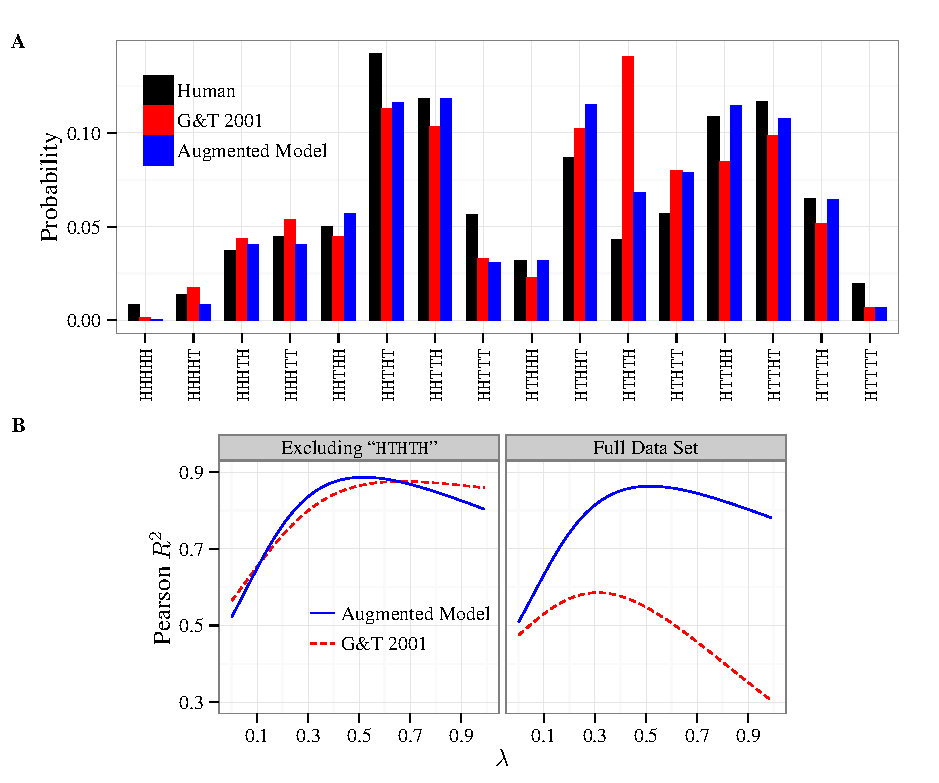
\includegraphics[scale=1]{RND-Figs/Fig2}
  \caption{\textbf{A}. Bayesian models fitting to human data in random sequence production. Human data represent the responses of $20,\!099$ participants \cite{Goodfellow1938}.
  In the model by Griffiths and Tenenbaum (2001), the bias-gain parameter $\lambda = 0.6$ was obtained by best-fitting to $15$ out of $16$ human data points (excluding ``\texttt{HTHTH}'').
  In the augmented model, $\lambda = 0.51$ was derived from the emergent behavior of the neural model (Equation~\ref{eq:lambda-by-RA}).
  \textbf{B}. Best-fitting $\lambda$ values for the model by Griffiths and Tenenbaum (2001) and the augmented model, with either the selected or full data set.
  Note that in both data sets, the optimal $\lambda$ value for the augmented model remains the same at $0.51$ as predicted by the neural model.
  }
  \label{fig2}
\end{figure}

\vskip6pt

Next, we asked whether it was possible to relate this emergent behavior of the neural model to an existing Bayesian model of randomness judgments by Griffiths and Tenenbaum (2001) \cite{Griffiths2001}.
This model was fit to a massive database from the ``Zenith radio experiment'', where $20,\!099$ participants attempted to produce $5$ random binary symbols one at a time, but nevertheless showed an apparent bias toward alternations \cite{Goodfellow1938}.
To account for such a bias, the Bayesian model included a bias-gain parameter $\lambda$ that weights the contribution of a local representativeness function ($L_k$) in determining the probability of the $k^{th}$ response ($R_k$) in a sequence being heads,

\begin{equation}\label{eq:model-GT2001}   %% Griffiths2001cogsci-eq7-8
    P(R_k = \mathtt{H}) = \frac{1}{1+e^{-\lambda L_k}}
\end{equation}
where $L_k$ is the log-likelihood by which choosing \texttt{H} instead of \texttt{T} at $R_k$ would make the sequence $\{R_1, \ldots, R_k\}$ appear more ``random'', based on the numbers of heads ($H$) and tails ($T$) from the prior responses $\{R_1, \ldots, R_{k-1}\}$,
\begin{equation}\label{eq:log-likelihood-L} %%% {eq:Griffiths2001cogsci-eq6}
  L_k = \log \prod_{i=1}^{k-1} \left(\frac{T_i + 1}{H_i + 1} \right), \quad k \geq 2
\end{equation}

Apparently, the bias-gain parameter $\lambda$ in Equation~\ref{eq:model-GT2001} modulates the strength of the alternation bias ---
a value of $\lambda=0$ produces ``unbiased'' judgments,
$P(R_k = \mathtt{H}) = 1/2$ regardless of the history,
in accord with the mean time statistic and the true probability of alternation $p_A=1/2$;
And, higher values $\lambda>0$ produce an increasing alternation bias, $P(R_{k} = \mathtt{H} |R_{k-1} = \mathtt{H}) < 1/2$.
%%ROR 0815: ``rational'' judgments.
Griffiths and Tenenbaum (2001) found that a $\lambda$ value of around $0.6$ produced the optimal fit to $15$ out of the $16$ data points from the human data (\textbf{Figure~2A}) --- a moderate alternation bias.
But they had no independent basis for specifying this value, beyond parameter fitting.
In contrast, we are able to show that $\lambda$ can be derived directly from the behavior of our neural model.

Specifically, from Equations \ref{eq:subjective-pa} and \ref{eq:model-GT2001}, we can derive $\lambda$ directly from the $R/A$ ratio:
\begin{equation}\label{eq:lambda-by-RA}
  \lambda = - \log_2(R/A)
\end{equation}
For independent fair coin flipping (i.e., $p_A=1/2$), the neural model showed $R/A \approx .7$, resulting in $\lambda \approx 0.51$ ---
precisely the value that optimizes the fit to the human data (\textbf{Figure~2B}).
%% YS: if we use ``precisely'' here (in ROR 0815), we are already talking about the augmented model, fitting to either the selected or the full data set, with the same lambda
Thus, by using the naturally emergent behavior of the neural model, we can independently anchor this previously free parameter, and obtain the best fit to the human data.
In addition, Equation~\ref{eq:lambda-by-RA} demonstrates that $\lambda$ is in accord with the subjective probability of alternation $p'_A$ (Equation~\ref{eq:subjective-pa}),
and normatively, the ratio of the combined mean and waiting time statistics (Equation~\ref{eq:time-ratio-squared}).
This represents a remarkable convergence across multiple levels of analysis, and further bolsters the validity of our understanding for the nature and origin of the systematic preference for alternating sequences, and against repeating ones.

Finally, the model by Griffiths and Tenenbaum (2001) produced a very bad fit to one of the sequences: \texttt{HTHTH}, which was judged by people to not be a very good random sequence, but the model ranked it highly.
It seems that people also have a bias against repeating the higher-order pattern events (e.g., $2$ consecutive alternations in \texttt{HTH}).
We were able to add this bias into the model as an additional additive term ($M_k$) in Equation~\ref{eq:model-GT2001},
\begin{equation}\label{eq:model-augmented}
  P(R_k = \mathtt{H}) = \frac{1}{1+e^{-\lambda (L_k + M_k)}}
\end{equation}
where $M_k$ performs a similar function as $L_k$, except being based on the numbers of the second-order pattern events, $O_{\mathtt{H}}$ and $O_{\mathtt{T}}$ (either alternation or repetition depending the choice at $R_{k-1}$),
\begin{equation}\label{eq:log-likelihood-M}
  M_k = \log \left(\frac{O_{\mathtt{T}} + 1}{O_{\mathtt{H}} + 1} \right), \quad k \geq 3
\end{equation}
This augmented model now produces an excellent fit to the full set of sequence data points (\textbf{Figure~2}).
Again, the optimal value of the bias-gain parameter $\lambda$, which now applies to both sources of bias, is the same $0.51$ value predicted by our neural model.
%(To obtain the $\lambda$ value for higher-order pattern events, we can use the same neural model by simply replacing the training symbols, e.g., replacing \texttt{HH} and \texttt{TT} with \texttt{R}, and replacing \texttt{HT} and \texttt{TH} with \texttt{A}.)

\vskip6pt

In conclusion, we find that the latent structure in simple probabilistic sequences shapes the learning dynamics in a neural model, producing a novel ``rational'' explanation for what has generally been considered a curious failure of human probabilistic understanding.
The remarkable fit of the parameters derived from this neural model with a Bayesian model derived from very different considerations reinforces the idea that the temporal integration mechanisms in our neural model provide a good account of human information integration over time.
We have also recently shown how this same neural temporal integration and learning framework can account for human causal learning \cite{OReilly2014blicket}, in a way that is also compatible with existing Bayesian models of causal reasoning \cite{Griffiths2010TiCS}.
This ability to bridge between levels of analysis across multiple domains represents a rare and important development, with the potential to both ground these abstract models in underlying neural mechanisms, and provide a simpler explanatory understanding of the emergent behavior of these neural models.




\bibliography{RND}

\bibliographystyle{Science}


\begin{scilastnote}
\item Acknowledgments
\end{scilastnote}


\end{document}
